\input{header}

\AtBeginSubsection[]
{
	\begin{frame}<beamer>
		\frametitle{Outline}
		\tableofcontents[current,currentsubsection]
	\end{frame}
}

\begin{document}

\begin{frame}[allowframebreaks] \frametitle{Decidability and CFL}
  \begin{itemize}
\item Acceptance problem of CFG
  \begin{equation*}
    A_{CFG}
=\{\langle  G,w\rangle \mid
G: CFG,\mbox{ generates } w\}
  \end{equation*}
\item We prove that $A_{CFG}$ is decidable
\item But an issue is the $\infty$ possible derivations of a CFG

\item For example,
  \begin{equation*}
  A\rightarrow B, B \rightarrow A
\end{equation*}

\item Chomsky normal form
  \begin{eqnarray*}
    && A \rightarrow BC\\
&& A \rightarrow a
  \end{eqnarray*}

\item Any $w, |w|=n$, derivation in 
exactly $2n-1$ steps

\item If $q$ is the \# rules, check all $q^{2n-1}$ branches

\item Proof
  \begin{enumerate}
  \item Convert $G$ to Chomsky
  \item Check all $q^{2n-1}$ branches
  \end{enumerate}

\item Results apply to PDA as well: for PDA we have a finite
  procedure to generate a CFG.
\end{itemize}\end{frame}

\begin{frame}[allowframebreaks] \frametitle{$E_{CFG}$}
\begin{equation*}
  E_{CFG}
=\{\langle  G\rangle \mid
G: CFG, L(G)=\emptyset\}
\end{equation*}
  \begin{itemize}
  \item idea: bottom up setting to see if any string can be generated
    from the start variable. From
  \begin{equation*}
    A\rightarrow a
  \end{equation*}
  We search if there is a rule
\begin{equation*}
  B\rightarrow A
\end{equation*}

\item Proof:
  \begin{enumerate}
  \item Mark all terminals
  \item Repeat until no new variables are marked

  \item [] \quad if
    \begin{equation*}
    A\rightarrow U_1\cdots U_k
  \end{equation*}
   \quad and 
   \begin{equation*}
\text{all }    U_1, \ldots, U_k \text{ marked}
 \end{equation*}
\quad $\Rightarrow$  mark $A$
\item If start variable is not marked, accept
\item [] Otherwise, reject
  \end{enumerate}
\item Number of iterations is finite: bounded by the number of
  variables
\item Each iteration is a finite procedure: we check all rules
\end{itemize}\end{frame} \begin{frame}[allowframebreaks] \frametitle{$EQ_{CFG}$}
\begin{equation*}
  EQ_{CFG}
=\{\langle  G,H\rangle \mid G,H: CFG, L(G)=
L(H)\}
\end{equation*}
  \begin{itemize}
\item Remember that $EQ_{DFA}$ is decidable
\item However, we cannot apply the same proof as
 CFL is not closed for 
$\cap$ and complementation
\item It's proved in Chapter 5 that this language is not decidable
\item We do not discuss details
\end{itemize}\end{frame}

\begin{frame}[allowframebreaks] \frametitle{CFL decidable}
  \begin{itemize}
\item This question is different from $A_{CFG}$ decidable
or not
\item How about converting PDA to a TM?
\item For nondeterministic PDA we can do NTM 
\item But nondeterministic PDA may have $\infty$-long branches

\item [] TM runs forever
\item So converting PDA to TM does not really work
\item A proof that works:

\item [] Find grammar $G$ for this CFL
\item [] Run TM for $\langle  G,w\rangle $ by using 
$A_{CFG}$
\end{itemize}\end{frame}

\begin{frame}[allowframebreaks] \frametitle{Classes of languages}
  \begin{itemize}
  \item Fig 4.10

\begin{center}
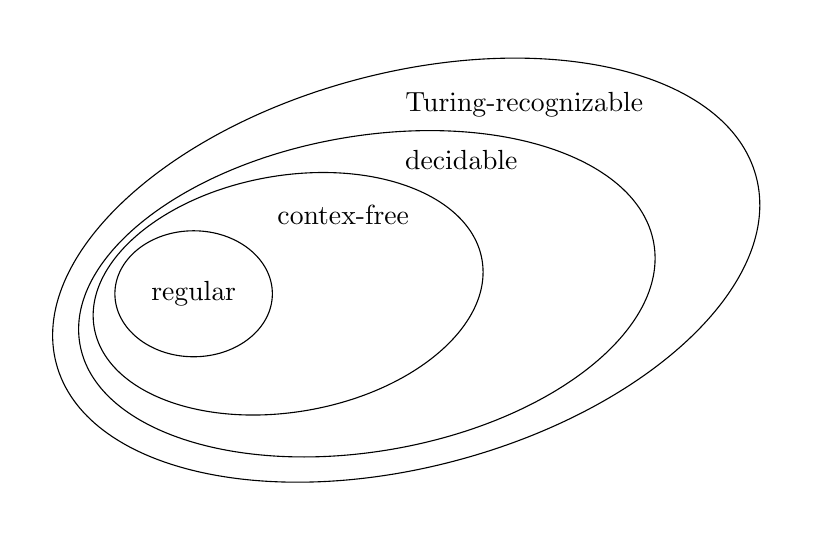
\begin{tikzpicture}
  % \draw (1,0) circle [radius=1.5];
  \draw (-3,0.3) circle [x radius=4.6cm, y radius=2.5cm, rotate=15];
  \draw (-3.5,0) circle [x radius=3.7cm, y radius=2cm, rotate=10];
  \draw (-4.5,0) circle [x radius=2.5cm, y radius=1.5cm, rotate=10];
  \draw (-5.7,0) circle [x radius=1cm, y radius=0.8cm];
  \path (-5.7,0) node {regular};
  \path (-3.8,1) node {contex-free};
  \path (-2.3,1.7) node {decidable};
  \path (-1.5,2.4) node {Turing-recognizable};  
\end{tikzpicture}
    \end{center}
  \end{itemize}\end{frame}

\end{document}

%%% Local Variables:
%%% mode: latex
%%% TeX-master: t
%%% End:
